\documentclass[twoside]{book}

% Packages required by doxygen
\usepackage{fixltx2e}
\usepackage{calc}
\usepackage{doxygen}
\usepackage[export]{adjustbox} % also loads graphicx
\usepackage{graphicx}
\usepackage[utf8]{inputenc}
\usepackage{makeidx}
\usepackage{multicol}
\usepackage{multirow}
\PassOptionsToPackage{warn}{textcomp}
\usepackage{textcomp}
\usepackage[nointegrals]{wasysym}
\usepackage[table]{xcolor}

% Font selection
\usepackage[T1]{fontenc}
\usepackage[scaled=.90]{helvet}
\usepackage{courier}
\usepackage{amssymb}
\usepackage{sectsty}
\renewcommand{\familydefault}{\sfdefault}
\allsectionsfont{%
  \fontseries{bc}\selectfont%
  \color{darkgray}%
}
\renewcommand{\DoxyLabelFont}{%
  \fontseries{bc}\selectfont%
  \color{darkgray}%
}
\newcommand{\+}{\discretionary{\mbox{\scriptsize$\hookleftarrow$}}{}{}}

% Page & text layout
\usepackage{geometry}
\geometry{%
  a4paper,%
  top=2.5cm,%
  bottom=2.5cm,%
  left=2.5cm,%
  right=2.5cm%
}
\tolerance=750
\hfuzz=15pt
\hbadness=750
\setlength{\emergencystretch}{15pt}
\setlength{\parindent}{0cm}
\setlength{\parskip}{3ex plus 2ex minus 2ex}
\makeatletter
\renewcommand{\paragraph}{%
  \@startsection{paragraph}{4}{0ex}{-1.0ex}{1.0ex}{%
    \normalfont\normalsize\bfseries\SS@parafont%
  }%
}
\renewcommand{\subparagraph}{%
  \@startsection{subparagraph}{5}{0ex}{-1.0ex}{1.0ex}{%
    \normalfont\normalsize\bfseries\SS@subparafont%
  }%
}
\makeatother

% Headers & footers
\usepackage{fancyhdr}
\pagestyle{fancyplain}
\fancyhead[LE]{\fancyplain{}{\bfseries\thepage}}
\fancyhead[CE]{\fancyplain{}{}}
\fancyhead[RE]{\fancyplain{}{\bfseries\leftmark}}
\fancyhead[LO]{\fancyplain{}{\bfseries\rightmark}}
\fancyhead[CO]{\fancyplain{}{}}
\fancyhead[RO]{\fancyplain{}{\bfseries\thepage}}
\fancyfoot[LE]{\fancyplain{}{}}
\fancyfoot[CE]{\fancyplain{}{}}
\fancyfoot[RE]{\fancyplain{}{\bfseries\scriptsize Generated by Doxygen }}
\fancyfoot[LO]{\fancyplain{}{\bfseries\scriptsize Generated by Doxygen }}
\fancyfoot[CO]{\fancyplain{}{}}
\fancyfoot[RO]{\fancyplain{}{}}
\renewcommand{\footrulewidth}{0.4pt}
\renewcommand{\chaptermark}[1]{%
  \markboth{#1}{}%
}
\renewcommand{\sectionmark}[1]{%
  \markright{\thesection\ #1}%
}

% Indices & bibliography
\usepackage{natbib}
\usepackage[titles]{tocloft}
\setcounter{tocdepth}{3}
\setcounter{secnumdepth}{5}
\makeindex

% Hyperlinks (required, but should be loaded last)
\usepackage{ifpdf}
\ifpdf
  \usepackage[pdftex,pagebackref=true]{hyperref}
\else
  \usepackage[ps2pdf,pagebackref=true]{hyperref}
\fi
\hypersetup{%
  colorlinks=true,%
  linkcolor=blue,%
  citecolor=blue,%
  unicode%
}

% Custom commands
\newcommand{\clearemptydoublepage}{%
  \newpage{\pagestyle{empty}\cleardoublepage}%
}

\usepackage{caption}
\captionsetup{labelsep=space,justification=centering,font={bf},singlelinecheck=off,skip=4pt,position=top}

%===== C O N T E N T S =====

\begin{document}

% Titlepage & ToC
\hypersetup{pageanchor=false,
             bookmarksnumbered=true,
             pdfencoding=unicode
            }
\pagenumbering{alph}
\begin{titlepage}
\vspace*{7cm}
\begin{center}%
{\Large My Project }\\
\vspace*{1cm}
{\large Generated by Doxygen 1.8.14}\\
\end{center}
\end{titlepage}
\clearemptydoublepage
\pagenumbering{roman}
\tableofcontents
\clearemptydoublepage
\pagenumbering{arabic}
\hypersetup{pageanchor=true}

%--- Begin generated contents ---
\chapter{Hierarchical Index}
\section{Class Hierarchy}
This inheritance list is sorted roughly, but not completely, alphabetically\+:\begin{DoxyCompactList}
\item Mono\+Behaviour\begin{DoxyCompactList}
\item \contentsline{section}{Bandit\+Car\+Behaviour}{\pageref{class_bandit_car_behaviour}}{}
\item \contentsline{section}{Bomb}{\pageref{class_bomb}}{}
\item \contentsline{section}{Bonuses}{\pageref{class_bonuses}}{}
\item \contentsline{section}{Bonus\+Spawner}{\pageref{class_bonus_spawner}}{}
\item \contentsline{section}{Car\+Controll}{\pageref{class_car_controll}}{}
\item \contentsline{section}{Car\+Durability\+Manager}{\pageref{class_car_durability_manager}}{}
\item \contentsline{section}{Civil\+Car\+Behavior}{\pageref{class_civil_car_behavior}}{}
\item \contentsline{section}{Civil\+Car\+Spawner}{\pageref{class_civil_car_spawner}}{}
\item \contentsline{section}{Infinite\+Road}{\pageref{class_infinite_road}}{}
\item \contentsline{section}{Shield}{\pageref{class_shield}}{}
\end{DoxyCompactList}
\end{DoxyCompactList}

\chapter{Class Index}
\section{Class List}
Here are the classes, structs, unions and interfaces with brief descriptions\+:\begin{DoxyCompactList}
\item\contentsline{section}{\mbox{\hyperlink{class_bandit_car_behaviour}{Bandit\+Car\+Behaviour}} }{\pageref{class_bandit_car_behaviour}}{}
\item\contentsline{section}{\mbox{\hyperlink{class_bomb}{Bomb}} }{\pageref{class_bomb}}{}
\item\contentsline{section}{\mbox{\hyperlink{class_bonuses}{Bonuses}} }{\pageref{class_bonuses}}{}
\item\contentsline{section}{\mbox{\hyperlink{class_bonus_spawner}{Bonus\+Spawner}} }{\pageref{class_bonus_spawner}}{}
\item\contentsline{section}{\mbox{\hyperlink{class_car_controll}{Car\+Controll}} }{\pageref{class_car_controll}}{}
\item\contentsline{section}{\mbox{\hyperlink{class_car_durability_manager}{Car\+Durability\+Manager}} }{\pageref{class_car_durability_manager}}{}
\item\contentsline{section}{\mbox{\hyperlink{class_civil_car_behavior}{Civil\+Car\+Behavior}} }{\pageref{class_civil_car_behavior}}{}
\item\contentsline{section}{\mbox{\hyperlink{class_civil_car_spawner}{Civil\+Car\+Spawner}} }{\pageref{class_civil_car_spawner}}{}
\item\contentsline{section}{\mbox{\hyperlink{class_infinite_road}{Infinite\+Road}} }{\pageref{class_infinite_road}}{}
\item\contentsline{section}{\mbox{\hyperlink{class_shield}{Shield}} }{\pageref{class_shield}}{}
\end{DoxyCompactList}

\chapter{Class Documentation}
\hypertarget{class_bandit_car_behaviour}{}\section{Bandit\+Car\+Behaviour Class Reference}
\label{class_bandit_car_behaviour}\index{Bandit\+Car\+Behaviour@{Bandit\+Car\+Behaviour}}
Inheritance diagram for Bandit\+Car\+Behaviour\+:\begin{figure}[H]
\begin{center}
\leavevmode
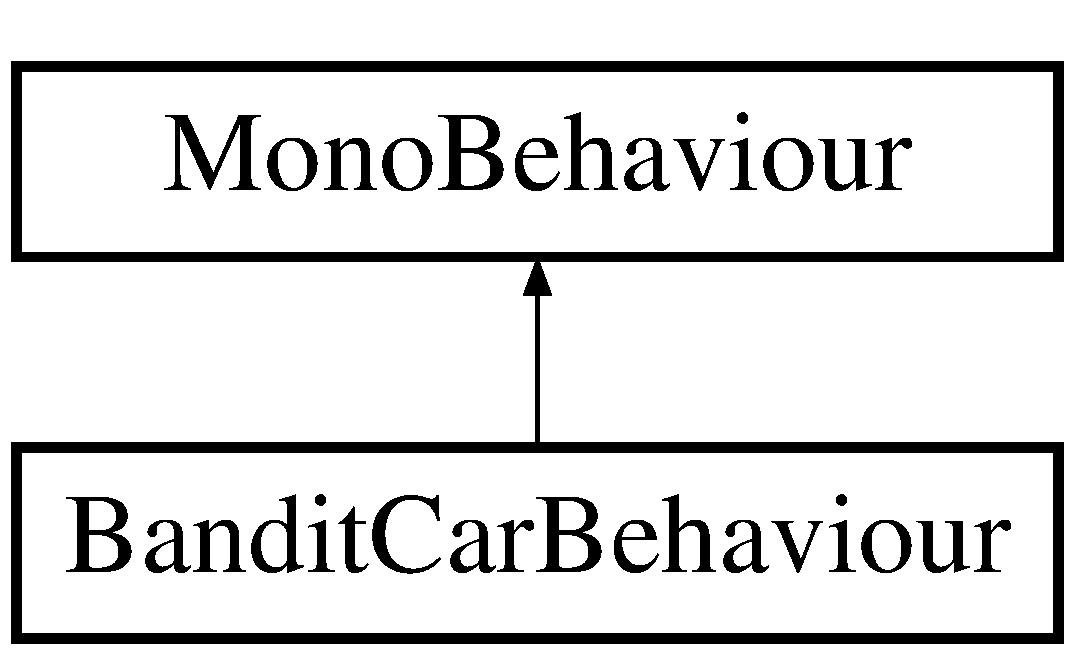
\includegraphics[height=2.000000cm]{class_bandit_car_behaviour}
\end{center}
\end{figure}
\subsection*{Public Attributes}
\begin{DoxyCompactItemize}
\item 
\mbox{\Hypertarget{class_bandit_car_behaviour_ae3b2699766531daf8718995e49cff662}\label{class_bandit_car_behaviour_ae3b2699766531daf8718995e49cff662}} 
Game\+Object {\bfseries bomb}
\item 
\mbox{\Hypertarget{class_bandit_car_behaviour_ad9ae8b1ef175f4105f1cd5b22ffdd4b4}\label{class_bandit_car_behaviour_ad9ae8b1ef175f4105f1cd5b22ffdd4b4}} 
int {\bfseries bombs\+Amount}
\item 
\mbox{\Hypertarget{class_bandit_car_behaviour_ac9802f2a6c5d6131364379c71e46c48f}\label{class_bandit_car_behaviour_ac9802f2a6c5d6131364379c71e46c48f}} 
int {\bfseries bandit\+Car\+Vertical\+Speed}
\item 
\mbox{\Hypertarget{class_bandit_car_behaviour_a698082f755c1bb892c7b28bbc37374d3}\label{class_bandit_car_behaviour_a698082f755c1bb892c7b28bbc37374d3}} 
int {\bfseries bandit\+Car\+Horizontal\+Speed}
\item 
\mbox{\Hypertarget{class_bandit_car_behaviour_a7d6ea6ee5ed41e1816340d7db49c00be}\label{class_bandit_car_behaviour_a7d6ea6ee5ed41e1816340d7db49c00be}} 
float {\bfseries bomb\+Delay}
\end{DoxyCompactItemize}


The documentation for this class was generated from the following file\+:\begin{DoxyCompactItemize}
\item 
Bandit\+Car\+Behaviour.\+cs\end{DoxyCompactItemize}

\hypertarget{class_bomb}{}\section{Bomb Class Reference}
\label{class_bomb}\index{Bomb@{Bomb}}
Inheritance diagram for Bomb\+:\begin{figure}[H]
\begin{center}
\leavevmode
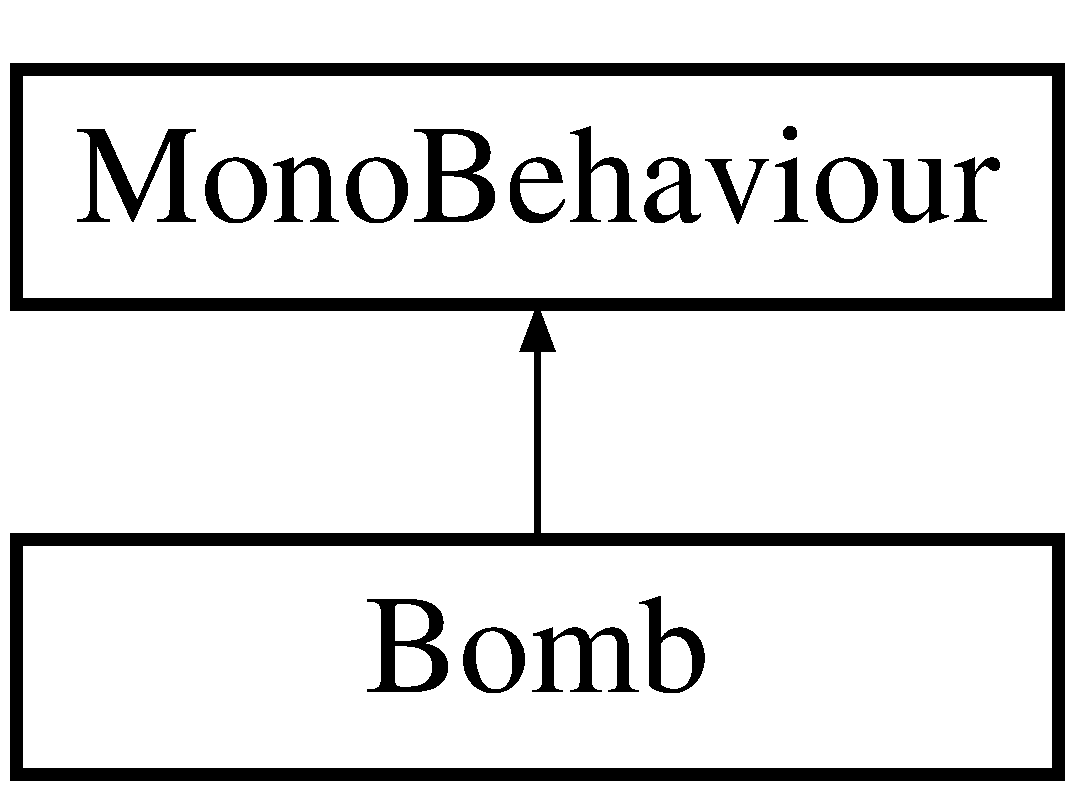
\includegraphics[height=2.000000cm]{class_bomb}
\end{center}
\end{figure}
\subsection*{Public Attributes}
\begin{DoxyCompactItemize}
\item 
\mbox{\Hypertarget{class_bomb_ac00ec933c991f5e1d89cb0409795ec95}\label{class_bomb_ac00ec933c991f5e1d89cb0409795ec95}} 
int {\bfseries bomb\+Dmg}
\item 
\mbox{\Hypertarget{class_bomb_a8b4b5c89e9e4de537c5f40478bf93fbb}\label{class_bomb_a8b4b5c89e9e4de537c5f40478bf93fbb}} 
float {\bfseries bomb\+Speed}
\end{DoxyCompactItemize}


The documentation for this class was generated from the following file\+:\begin{DoxyCompactItemize}
\item 
Bomb.\+cs\end{DoxyCompactItemize}

\hypertarget{class_bonuses}{}\section{Bonuses Class Reference}
\label{class_bonuses}\index{Bonuses@{Bonuses}}
Inheritance diagram for Bonuses\+:\begin{figure}[H]
\begin{center}
\leavevmode
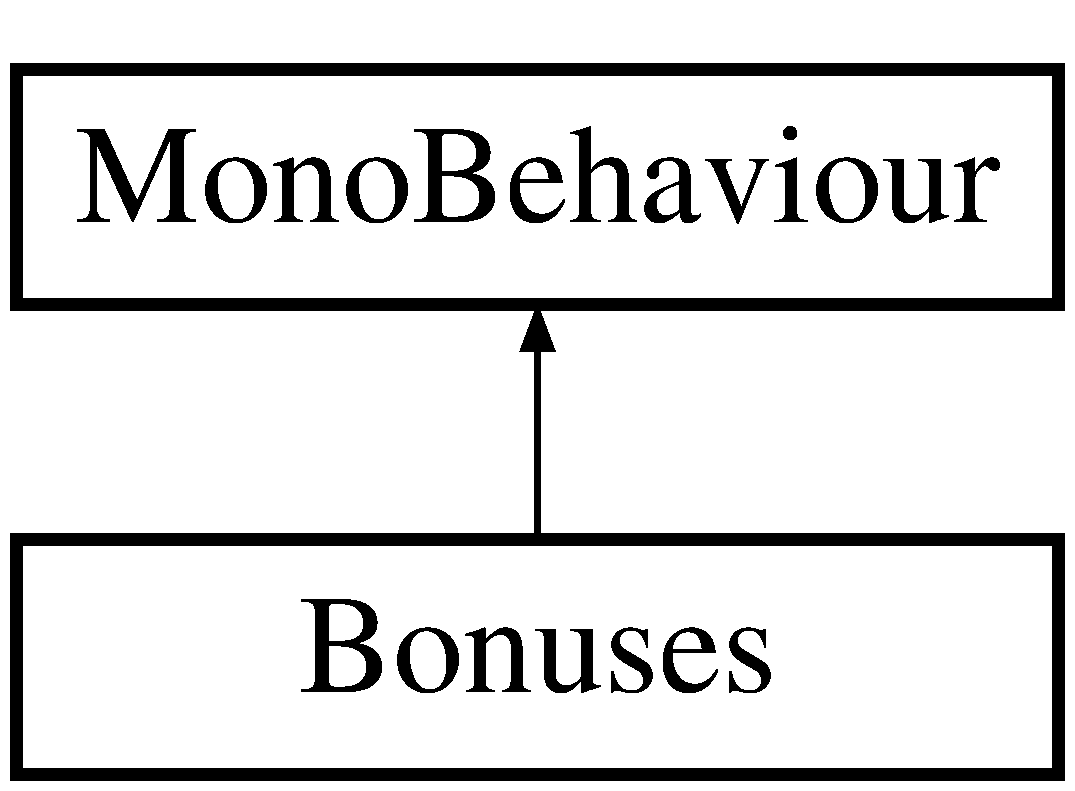
\includegraphics[height=2.000000cm]{class_bonuses}
\end{center}
\end{figure}
\subsection*{Public Attributes}
\begin{DoxyCompactItemize}
\item 
\mbox{\Hypertarget{class_bonuses_afe2f71cc039f782d99325f5034d5dc6f}\label{class_bonuses_afe2f71cc039f782d99325f5034d5dc6f}} 
bool {\bfseries is\+Durability}
\item 
\mbox{\Hypertarget{class_bonuses_a14a12d54544b213cd1fc7e536a40b53a}\label{class_bonuses_a14a12d54544b213cd1fc7e536a40b53a}} 
bool {\bfseries is\+Shield}
\item 
\mbox{\Hypertarget{class_bonuses_af737fff61136a35760579a9817116657}\label{class_bonuses_af737fff61136a35760579a9817116657}} 
bool {\bfseries is\+Speed}
\item 
\mbox{\Hypertarget{class_bonuses_a90b84f4d53b68c7c29151717659d7f4d}\label{class_bonuses_a90b84f4d53b68c7c29151717659d7f4d}} 
float {\bfseries bonus\+Speed} = 5f
\item 
\mbox{\Hypertarget{class_bonuses_a6c83276a4ae0d07998cd049723cbef48}\label{class_bonuses_a6c83276a4ae0d07998cd049723cbef48}} 
float {\bfseries repair\+Points}
\item 
\mbox{\Hypertarget{class_bonuses_a0025ffcc6c6aa27643fdfde248fd7a32}\label{class_bonuses_a0025ffcc6c6aa27643fdfde248fd7a32}} 
Game\+Object {\bfseries shield}
\item 
\mbox{\Hypertarget{class_bonuses_a55df35b9b3fa8807e3d2ce052987f1c8}\label{class_bonuses_a55df35b9b3fa8807e3d2ce052987f1c8}} 
float {\bfseries speed\+Boost}
\item 
\mbox{\Hypertarget{class_bonuses_a15504bd5074dfb6e7e54d4a51849d8e1}\label{class_bonuses_a15504bd5074dfb6e7e54d4a51849d8e1}} 
float {\bfseries duration}
\end{DoxyCompactItemize}


The documentation for this class was generated from the following file\+:\begin{DoxyCompactItemize}
\item 
Bonuses.\+cs\end{DoxyCompactItemize}

\hypertarget{class_bonus_spawner}{}\section{Bonus\+Spawner Class Reference}
\label{class_bonus_spawner}\index{Bonus\+Spawner@{Bonus\+Spawner}}
Inheritance diagram for Bonus\+Spawner\+:\begin{figure}[H]
\begin{center}
\leavevmode
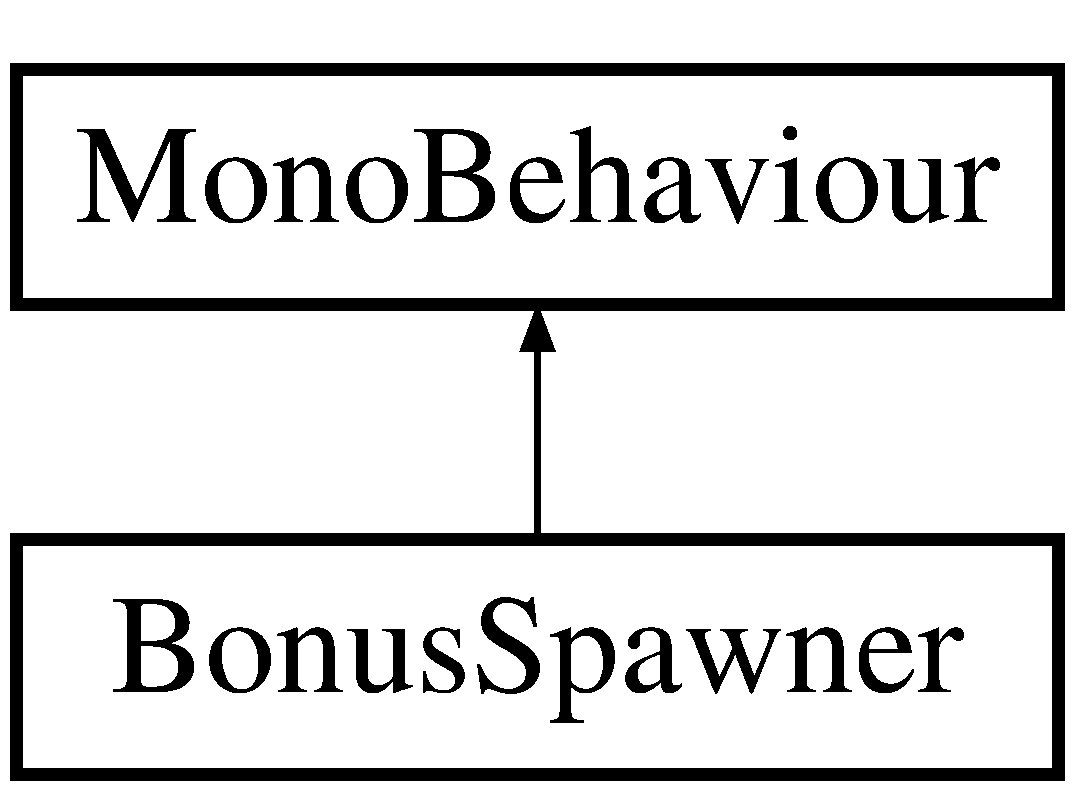
\includegraphics[height=2.000000cm]{class_bonus_spawner}
\end{center}
\end{figure}
\subsection*{Public Attributes}
\begin{DoxyCompactItemize}
\item 
\mbox{\Hypertarget{class_bonus_spawner_ad25c4d6982ce6c6320e82575edae417d}\label{class_bonus_spawner_ad25c4d6982ce6c6320e82575edae417d}} 
Game\+Object \mbox{[}$\,$\mbox{]} {\bfseries bonuses}
\item 
\mbox{\Hypertarget{class_bonus_spawner_a175114204cf7db8557af8018b04f7283}\label{class_bonus_spawner_a175114204cf7db8557af8018b04f7283}} 
int {\bfseries min\+Delay}
\item 
\mbox{\Hypertarget{class_bonus_spawner_aa0aecdf16c51c0dcf62dd4e573f742be}\label{class_bonus_spawner_aa0aecdf16c51c0dcf62dd4e573f742be}} 
int {\bfseries max\+Delay}
\end{DoxyCompactItemize}


The documentation for this class was generated from the following file\+:\begin{DoxyCompactItemize}
\item 
Bonus\+Spawner.\+cs\end{DoxyCompactItemize}

\hypertarget{class_car_controll}{}\section{Car\+Controll Class Reference}
\label{class_car_controll}\index{Car\+Controll@{Car\+Controll}}
Inheritance diagram for Car\+Controll\+:\begin{figure}[H]
\begin{center}
\leavevmode
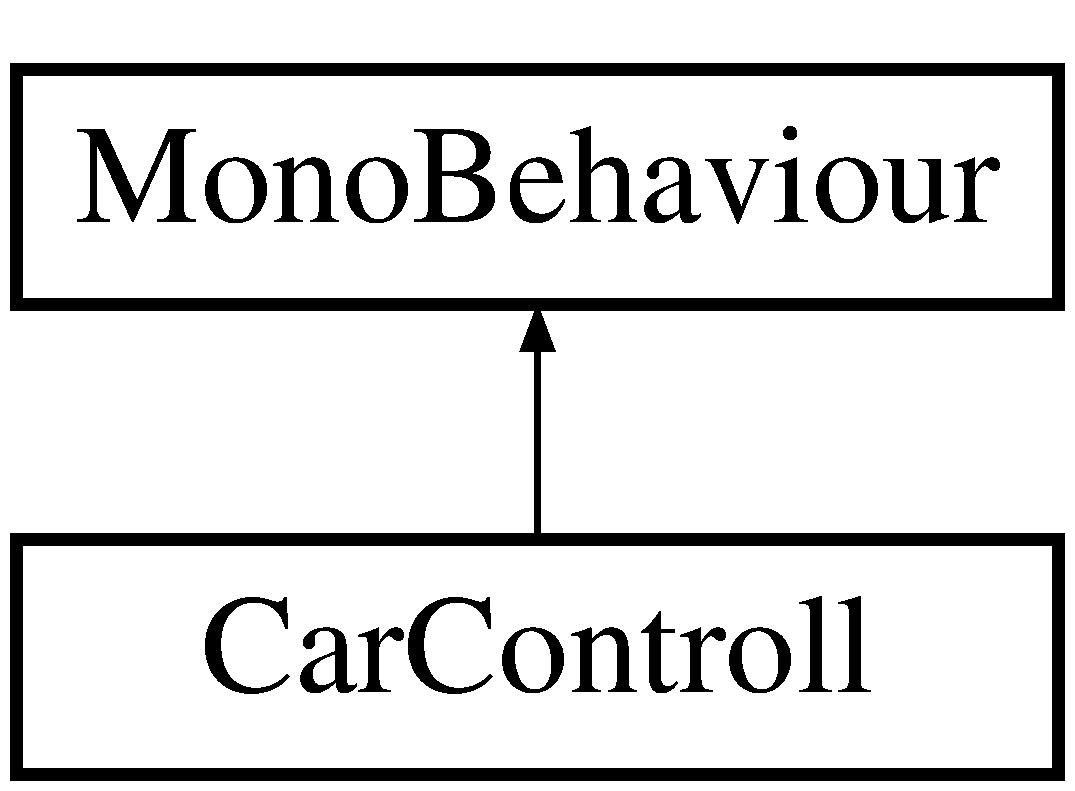
\includegraphics[height=2.000000cm]{class_car_controll}
\end{center}
\end{figure}
\subsection*{Public Member Functions}
\begin{DoxyCompactItemize}
\item 
\mbox{\Hypertarget{class_car_controll_ade3d6320b44eac1fcdc3907100c65f62}\label{class_car_controll_ade3d6320b44eac1fcdc3907100c65f62}} 
void {\bfseries Start} ()
\end{DoxyCompactItemize}
\subsection*{Public Attributes}
\begin{DoxyCompactItemize}
\item 
\mbox{\Hypertarget{class_car_controll_a21f57feb07197bd6b2c6d25c6480a195}\label{class_car_controll_a21f57feb07197bd6b2c6d25c6480a195}} 
float {\bfseries car\+Horizontal\+Speed}
\item 
\mbox{\Hypertarget{class_car_controll_a392570ecc618e5f4a8fbb6fe5e316b2d}\label{class_car_controll_a392570ecc618e5f4a8fbb6fe5e316b2d}} 
float {\bfseries max\+Durability} = 100f
\item 
\mbox{\Hypertarget{class_car_controll_a17e94e73ac019751ffdaf40f55ce8f50}\label{class_car_controll_a17e94e73ac019751ffdaf40f55ce8f50}} 
float {\bfseries durability}
\end{DoxyCompactItemize}


The documentation for this class was generated from the following file\+:\begin{DoxyCompactItemize}
\item 
Car\+Controll.\+cs\end{DoxyCompactItemize}

\hypertarget{class_car_durability_manager}{}\section{Car\+Durability\+Manager Class Reference}
\label{class_car_durability_manager}\index{Car\+Durability\+Manager@{Car\+Durability\+Manager}}
Inheritance diagram for Car\+Durability\+Manager\+:\begin{figure}[H]
\begin{center}
\leavevmode
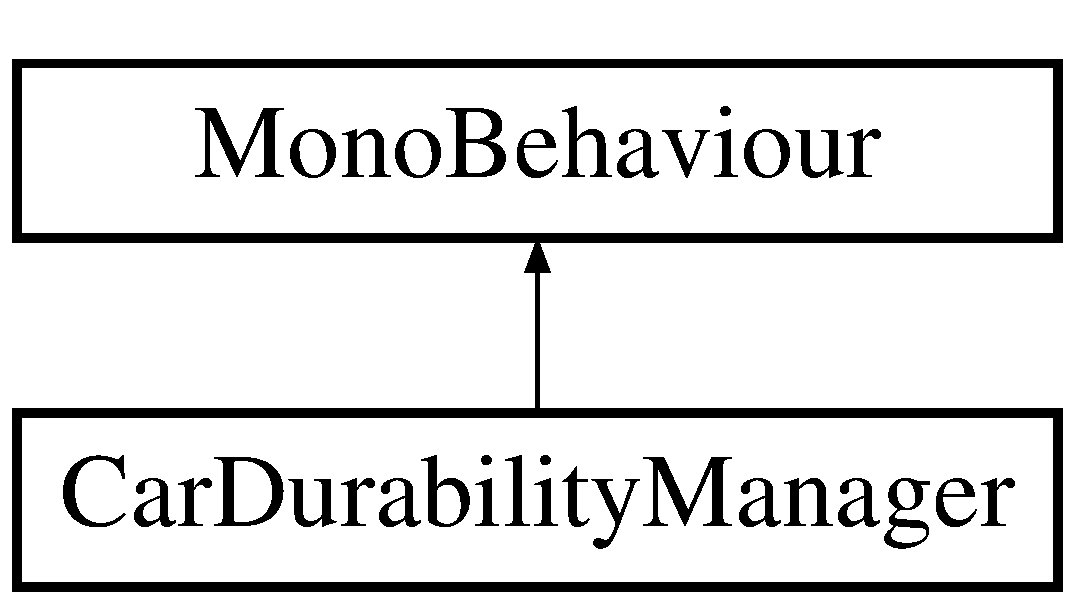
\includegraphics[height=2.000000cm]{class_car_durability_manager}
\end{center}
\end{figure}
\subsection*{Public Attributes}
\begin{DoxyCompactItemize}
\item 
\mbox{\Hypertarget{class_car_durability_manager_a409e9361daf37959c10b1688f83e2671}\label{class_car_durability_manager_a409e9361daf37959c10b1688f83e2671}} 
Game\+Object {\bfseries player\+Car\+Prefab}
\item 
\mbox{\Hypertarget{class_car_durability_manager_a2051dd135639e79ae89f3dda7700a7c3}\label{class_car_durability_manager_a2051dd135639e79ae89f3dda7700a7c3}} 
Game\+Object {\bfseries player\+Car\+Spawn\+Place}
\item 
\mbox{\Hypertarget{class_car_durability_manager_aa71c2564d7d5d5699fd5f3ed4925c534}\label{class_car_durability_manager_aa71c2564d7d5d5699fd5f3ed4925c534}} 
Text\+Mesh {\bfseries durability\+Text}
\item 
\mbox{\Hypertarget{class_car_durability_manager_ab5f76ce6be91794c08975d0b699d4ed0}\label{class_car_durability_manager_ab5f76ce6be91794c08975d0b699d4ed0}} 
int {\bfseries Nr\+Of\+Lifes}
\end{DoxyCompactItemize}


The documentation for this class was generated from the following file\+:\begin{DoxyCompactItemize}
\item 
Car\+Durability\+Manager.\+cs\end{DoxyCompactItemize}

\hypertarget{class_civil_car_behavior}{}\section{Civil\+Car\+Behavior Class Reference}
\label{class_civil_car_behavior}\index{Civil\+Car\+Behavior@{Civil\+Car\+Behavior}}
Inheritance diagram for Civil\+Car\+Behavior\+:\begin{figure}[H]
\begin{center}
\leavevmode
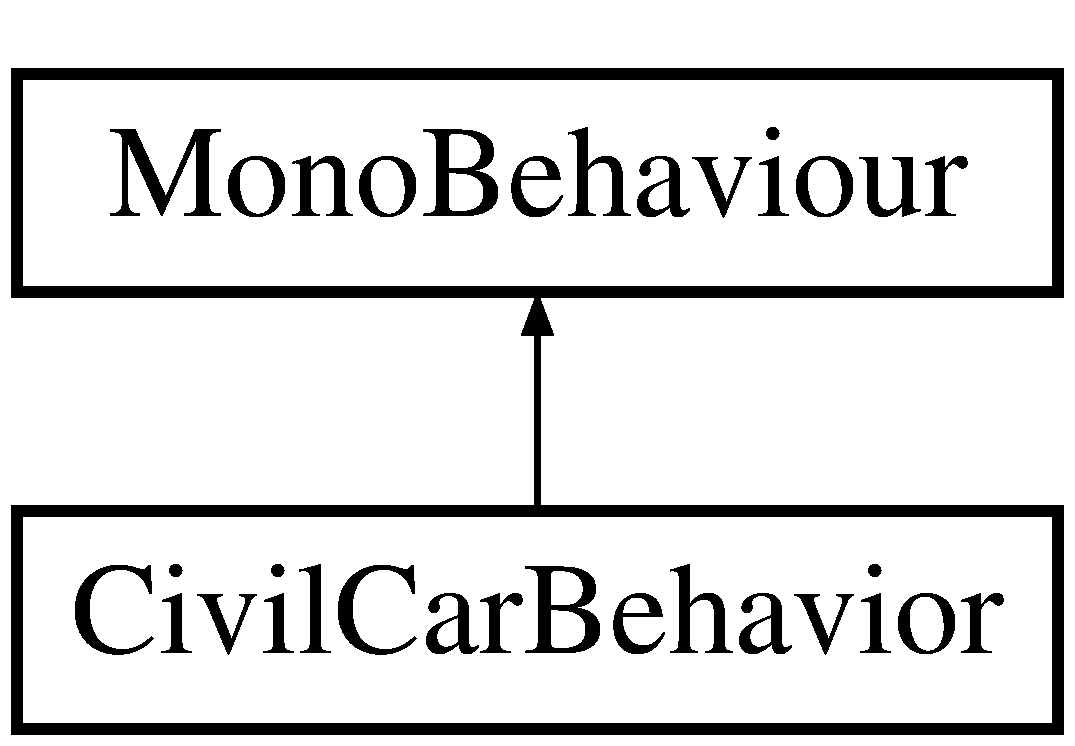
\includegraphics[height=2.000000cm]{class_civil_car_behavior}
\end{center}
\end{figure}
\subsection*{Public Attributes}
\begin{DoxyCompactItemize}
\item 
\mbox{\Hypertarget{class_civil_car_behavior_aebb222030998599113eb783dfc903fc4}\label{class_civil_car_behavior_aebb222030998599113eb783dfc903fc4}} 
float {\bfseries civil\+Car\+Speed}
\item 
\mbox{\Hypertarget{class_civil_car_behavior_a74149c796566b4900c6ecc677b02608e}\label{class_civil_car_behavior_a74149c796566b4900c6ecc677b02608e}} 
int {\bfseries direction} = -\/1
\item 
\mbox{\Hypertarget{class_civil_car_behavior_abff5edca11197e0f032e7b2ebd74aba2}\label{class_civil_car_behavior_abff5edca11197e0f032e7b2ebd74aba2}} 
float {\bfseries crash\+Damage} = 25f
\end{DoxyCompactItemize}


The documentation for this class was generated from the following file\+:\begin{DoxyCompactItemize}
\item 
Civil\+Car\+Behavior.\+cs\end{DoxyCompactItemize}

\hypertarget{class_civil_car_spawner}{}\section{Civil\+Car\+Spawner Class Reference}
\label{class_civil_car_spawner}\index{Civil\+Car\+Spawner@{Civil\+Car\+Spawner}}
Inheritance diagram for Civil\+Car\+Spawner\+:\begin{figure}[H]
\begin{center}
\leavevmode
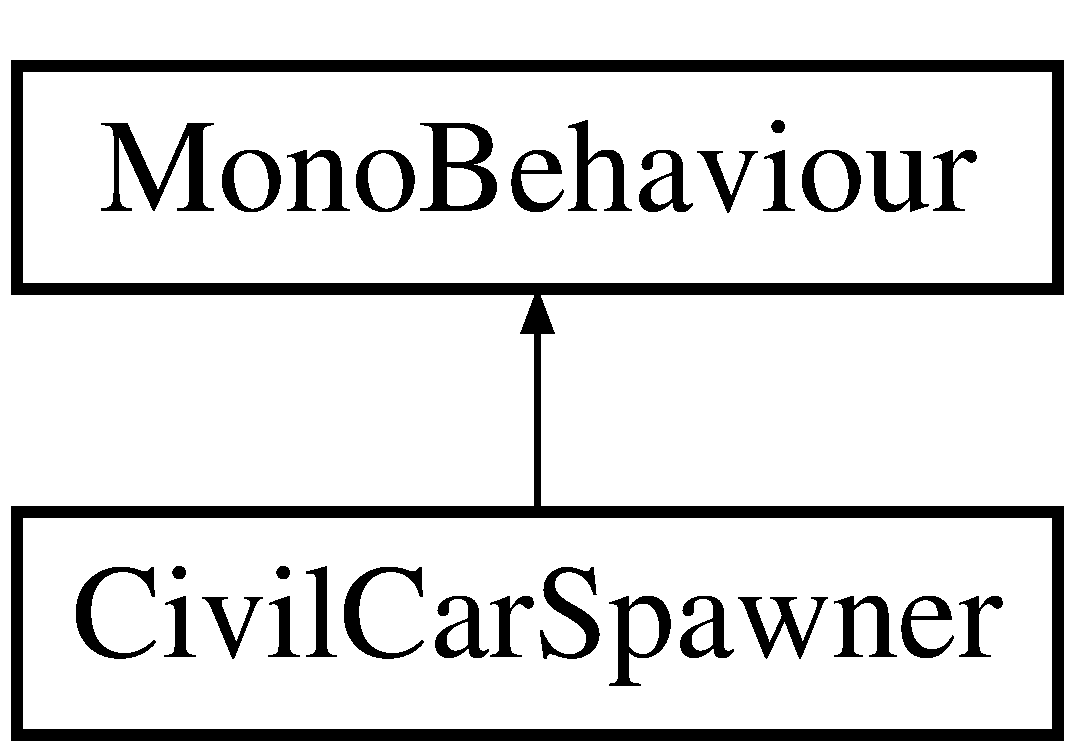
\includegraphics[height=2.000000cm]{class_civil_car_spawner}
\end{center}
\end{figure}
\subsection*{Public Attributes}
\begin{DoxyCompactItemize}
\item 
\mbox{\Hypertarget{class_civil_car_spawner_a073ee708a84ce77cdb3fe77b8d0437f8}\label{class_civil_car_spawner_a073ee708a84ce77cdb3fe77b8d0437f8}} 
float {\bfseries car\+Spawn\+Delay} = 4f
\item 
\mbox{\Hypertarget{class_civil_car_spawner_ab7010efa538bb073c7c66f77f7950b98}\label{class_civil_car_spawner_ab7010efa538bb073c7c66f77f7950b98}} 
Game\+Object {\bfseries civil\+Car}
\end{DoxyCompactItemize}


The documentation for this class was generated from the following file\+:\begin{DoxyCompactItemize}
\item 
Civil\+Car\+Spawner.\+cs\end{DoxyCompactItemize}

\hypertarget{class_infinite_road}{}\section{Infinite\+Road Class Reference}
\label{class_infinite_road}\index{Infinite\+Road@{Infinite\+Road}}
Inheritance diagram for Infinite\+Road\+:\begin{figure}[H]
\begin{center}
\leavevmode
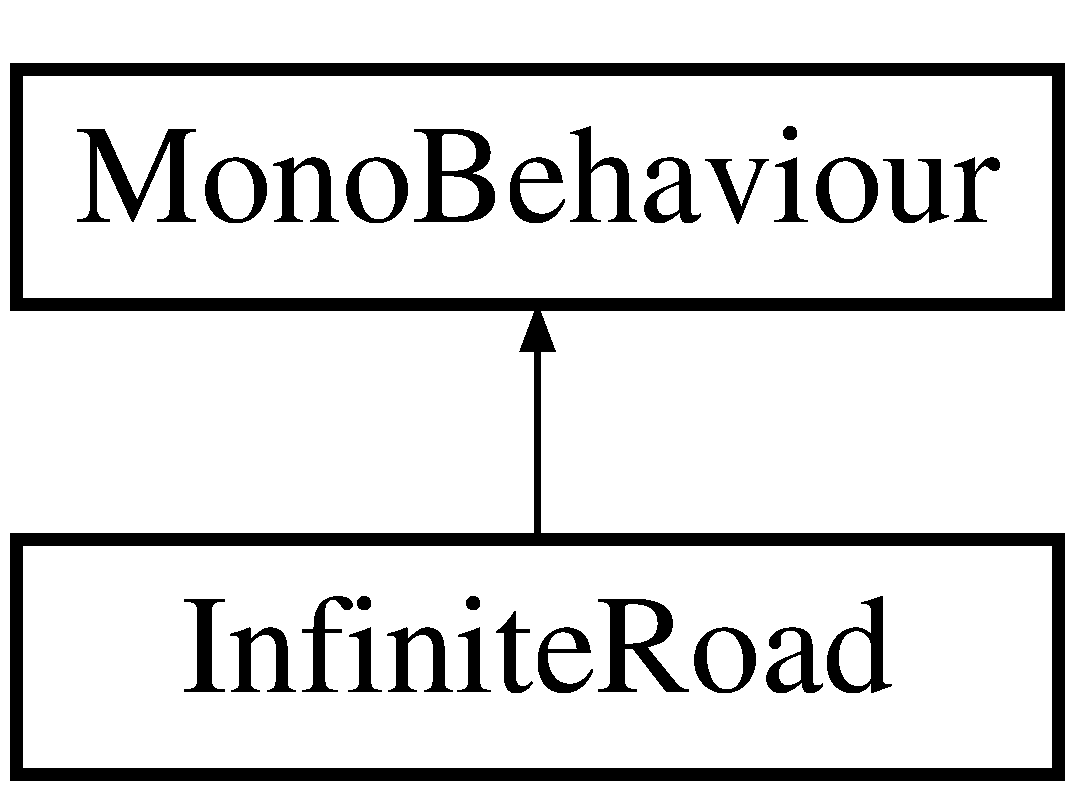
\includegraphics[height=2.000000cm]{class_infinite_road}
\end{center}
\end{figure}
\subsection*{Public Attributes}
\begin{DoxyCompactItemize}
\item 
\mbox{\Hypertarget{class_infinite_road_a8ec228236d13ed0064b5f29f2f3d6e91}\label{class_infinite_road_a8ec228236d13ed0064b5f29f2f3d6e91}} 
float {\bfseries scroll\+Speed}
\end{DoxyCompactItemize}


The documentation for this class was generated from the following file\+:\begin{DoxyCompactItemize}
\item 
Infinite\+Road.\+cs\end{DoxyCompactItemize}

\hypertarget{class_shield}{}\section{Shield Class Reference}
\label{class_shield}\index{Shield@{Shield}}
Inheritance diagram for Shield\+:\begin{figure}[H]
\begin{center}
\leavevmode
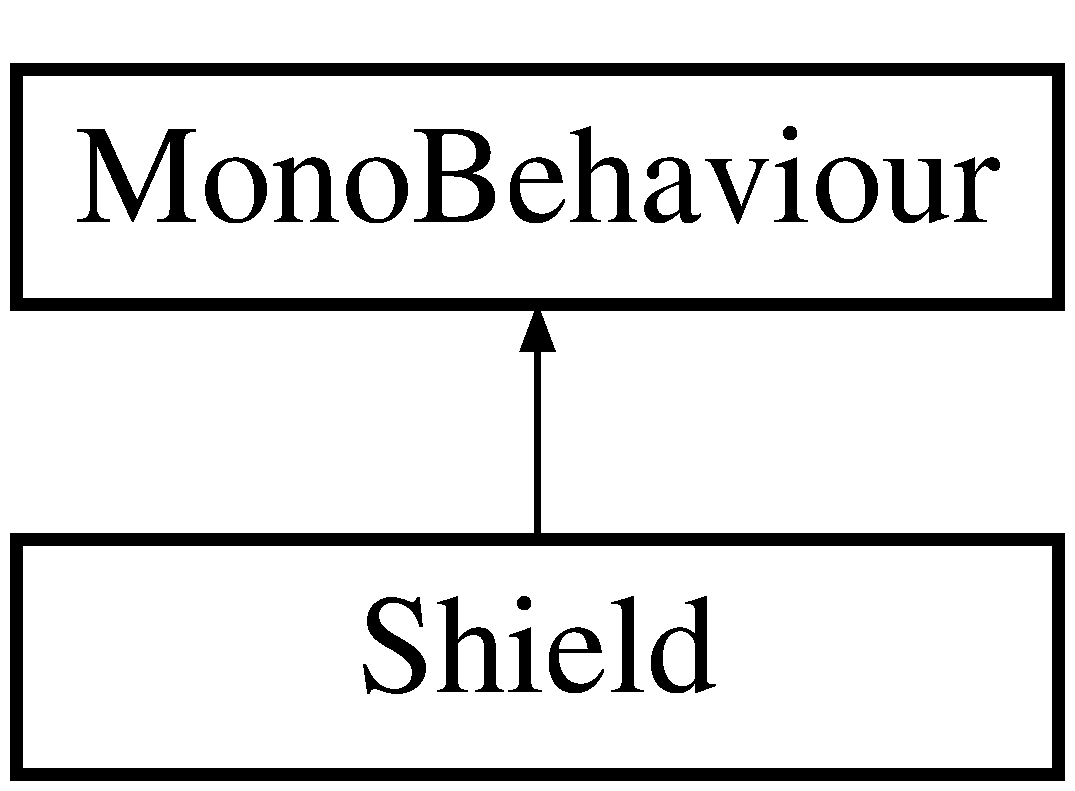
\includegraphics[height=2.000000cm]{class_shield}
\end{center}
\end{figure}
\subsection*{Public Attributes}
\begin{DoxyCompactItemize}
\item 
\mbox{\Hypertarget{class_shield_ac92a7a2922666b60af656d75f21b7d9a}\label{class_shield_ac92a7a2922666b60af656d75f21b7d9a}} 
float {\bfseries shield\+Duration}
\end{DoxyCompactItemize}


The documentation for this class was generated from the following file\+:\begin{DoxyCompactItemize}
\item 
Shield.\+cs\end{DoxyCompactItemize}

%--- End generated contents ---

% Index
\backmatter
\newpage
\phantomsection
\clearemptydoublepage
\addcontentsline{toc}{chapter}{Index}
\printindex

\end{document}
